%%%%%%%%%%%%%%%%%%%%%%%%%%%%%%%%%%%%%%%%%
% Beamer Presentation
% LaTeX Template
% Version 1.0 (10/11/12)
%
% This template has been downloaded from:
% http://www.LaTeXTemplates.com
%
% License:
% CC BY-NC-SA 3.0 (http://creativecommons.org/licenses/by-nc-sa/3.0/)
%
%%%%%%%%%%%%%%%%%%%%%%%%%%%%%%%%%%%%%%%%%

%----------------------------------------------------------------------------------------
%	PACKAGES AND THEMES
%----------------------------------------------------------------------------------------
%!TEX encoding = UTF-8 Unicode


\documentclass[12pt,handout]{beamer}
\usepackage[utf8]{inputenc}
\usepackage[T1]{fontenc}
\usepackage{verbatim}

\mode<presentation> {

\usetheme{Pittsburgh}

}

\usepackage{graphicx} % Allows including images
\usepackage{booktabs} % Allows the use of \toprule, \midrule and \bottomrule in tables

%----------------------------------------------------------------------------------------
%	TITLE PAGE
%----------------------------------------------------------------------------------------

\title[]{Critical behaviour of the surface tension in the 3D Ising model} % The short title appears at the bottom of every slide, the full title is only on the title page

\author[]
{
Federico Belliardo \\
Marco Costa
} 

\institute[] % Your institution as it will appear on the bottom of every slide, may be shorthand to save space
{
Dipartimento di Fisica\\ % Your institution for the title page
Università di Pisa \\
\medskip
}
\date{\today} % Date, can be changed to a custom date

\begin{document}

\begin{frame}
\titlepage % Print the title page as the first slide
\end{frame}

%\begin{frame}
%\frametitle{Overview} % Table of contents slide, comment this block out to remove it
%\tableofcontents % Throughout your presentation, if you choose to use \section{} and \subsection{} commands, these will automatically be printed on this slide as an overview of your presentation
%\end{frame}

%----------------------------------------------------------------------------------------
%	PRESENTATION SLIDES
%----------------------------------------------------------------------------------------

\begin{frame}{Summary}

\begin{center}

\begin{itemize}
\item Definition of the surface tension
\item Algorithm for generating the Markov chain
\item (Notes on the implementation?)
\item Estimation of the errors and autocorrelation
\item Fit of the free energy
\item Fit of the critical behaviour
\item Conclusion
\end{itemize}

\end{center}
\end{frame}

\begin{frame}{Definition of the surface tension}
\begin{center}


\begin{figure}[!htb]
\centering
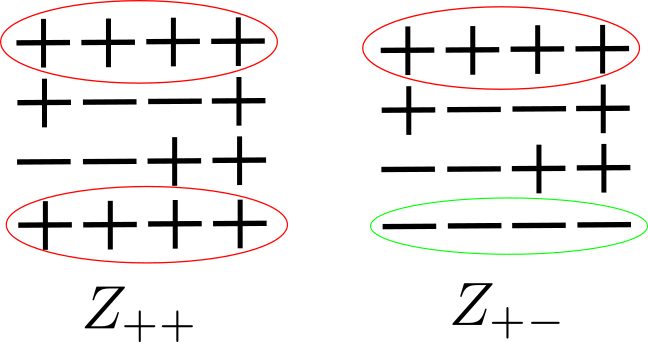
\includegraphics[scale=0.5]{bound.png}
\end{figure}

\large
\[
\sigma = \lim_{\substack{L \rightarrow +\infty \\  T \rightarrow +\infty}} \frac{1}{L^2} \log \frac{Z_{+-}}{Z_{++}}
\]

\note{L'ordine dei due limiti T e  non dovrebbe contare. Non so se si può "dimostrare" al nostro libello di rigore fisiamo T = 3L e facciamo il limite per L}

\note{$Z_{+-}$ e $Z_{++}$ sono le funzioni di partzione quando fisso cosa devono valere i layer di spin sul pavimento e sul soffito. Inserire piccola immagine per spiegarlo.}

\end{center}
\end{frame}

\begin{frame}{Definition of the surface tension}
\begin{center}
\[
\sigma = \lim_{\substack{L \rightarrow +\infty \\  T \rightarrow +\infty}} \frac{1}{L^2} \log \frac{Z_{+-}}{Z_{++}} = \frac{1}{L^2} \left( F_{+-} - F_{++} \right) 
\]

\
Free energy per area of the interface between phases.

\end{center}
\end{frame}

\begin{frame}{Definition of the surface tension}
\begin{center}



\begin{minipage}[t]{0.48\linewidth}
left part
\end{minipage}\hfill
\begin{minipage}[t]{0.48\linewidth}
\begin{figure}[!htb]
\centering
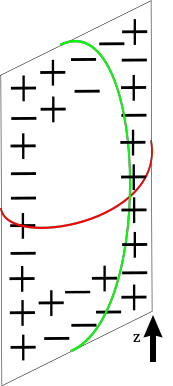
\includegraphics[scale=0.5]{antiferro.png}
\end{figure}
\end{minipage}

\end{center}
\end{frame}

\begin{frame}{Definition of the surface tension}
\begin{center}


\end{center}
\end{frame}


%----------------------------------------------------------------------------------------

\end{document} 